%!TEX root = thesis.tex
\chapter{Corner Transfer Matrix}
\label{chapter:ctm}
The \textit{cerner transfer matrix renormalization group} (CTMRG) \cite{} is an algorithm to numerically compute the \textit{effective environments} which is an approximation of the environment of systems. For example, if the infinite PEPS is composed by a single tensor $A^{h}_{uldr}$ repeatedly, where $h$ express a physical basis of  $\mathbb{V}$ with dimension $d$, and $u,l,d,r$ are virtual bonds with dimension $D$, see Fig. \ref{fig501}(a). Then we can represent the scale norm $\Braket{\psi|\psi}$ by a simple two dimensional tensor network $\varepsilon$ which is characterized by reduced tensors $a$, shown in Fig. \ref{fig501}(b). The reduced tensor $a$ is defined as eq.\ref{reduce_a}, 
\begin{align}
	\label{reduce_a}
	a \equiv \sum_{h=1}^{d} A_{h} \otimes A^{*}_{h}
\end{align}
The environment $\varepsilon^{[\vec{r}]}$ of the site $\vec{r}$ could be described by the reduced tensors in the gray rectangles in Fig.\ref{fig501}(c) and the \textit{effective environments} $G^{[\vec{r}]}$ shown in Fig. \ref{fig501}(d) is target of the CTMRG. 

In the following subsections, we will show more details of implementation of CTM and compare some features between obtaining the states from iPEPE and PESS.

\begin{figure}[ht]
	\centering
	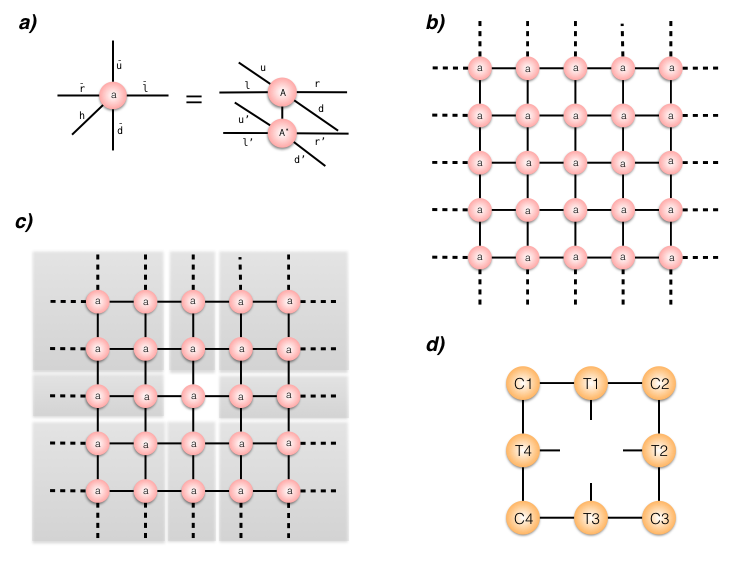
\includegraphics[width=0.75\textwidth]{figures/fig501.png}
	\caption[The picture of the main idea of itebd.]{The red and blue tensor denotes on \textit{odd} and \textit{even} sites. The yellow one are time evolution operators $e^{-\tau H_{k,k+1}}$, $e^{-\tau H_{k+1,k}}$}
	\label{fig501}
\end{figure}

\section{Obtain States from PEPS}
\label{2ditebdctm}
In chapter.\ref{chapter:2ditebd}, we have discussed about obtaining the infinite PEPS state $\Ket{\psi}$ of an infinite 2D square lattice by imaginary time evolution and knowing that the infinite PEPS could be characterized by two tensors A and B repeatedly. The state has components $A^d_{uldr}$ and $B^d_{drul}$. The label $d$ represent a physical basis and labels $u,l,d,r$ are the virtual bonds of infinite PEPS, Fig. \ref{fig511}(a). Next, for 

\begin{figure}[ht]
	\centering
	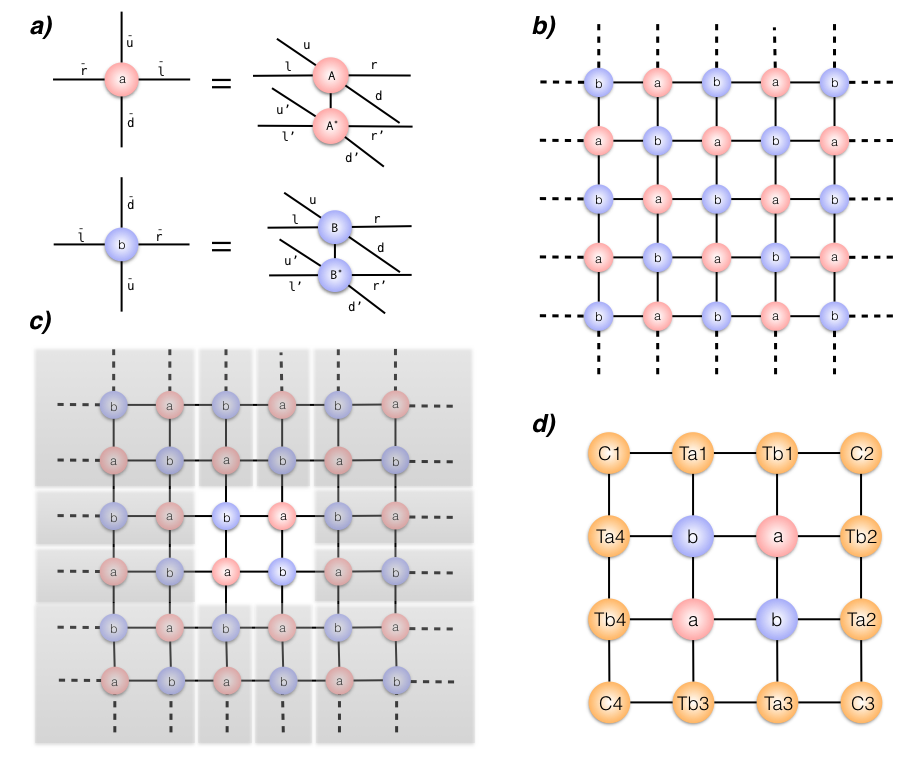
\includegraphics[width=0.75\textwidth]{figures/fig511.png}
	\caption[The picture of the main idea of itebd.]{The red and blue tensor denotes on \textit{odd} and \textit{even} sites. The yellow one are time evolution operators $e^{-\tau H_{k,k+1}}$, $e^{-\tau H_{k+1,k}}$}
	\label{fig511}
\end{figure}

\begin{figure}[ht]
	\centering
	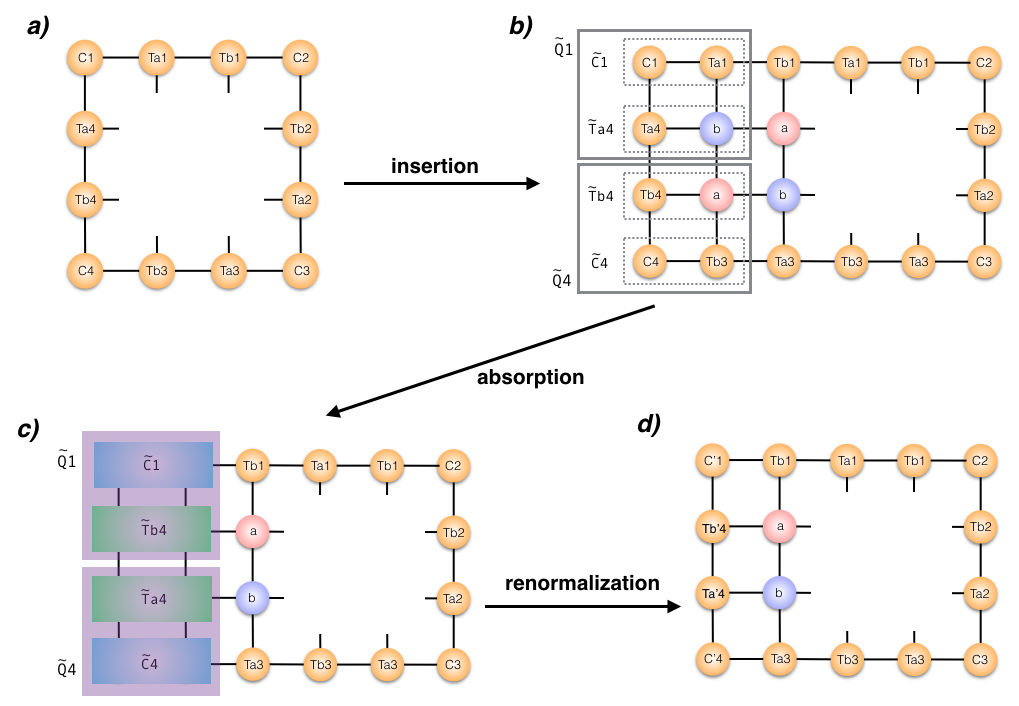
\includegraphics[width=0.75\textwidth]{figures/fig512.png}
	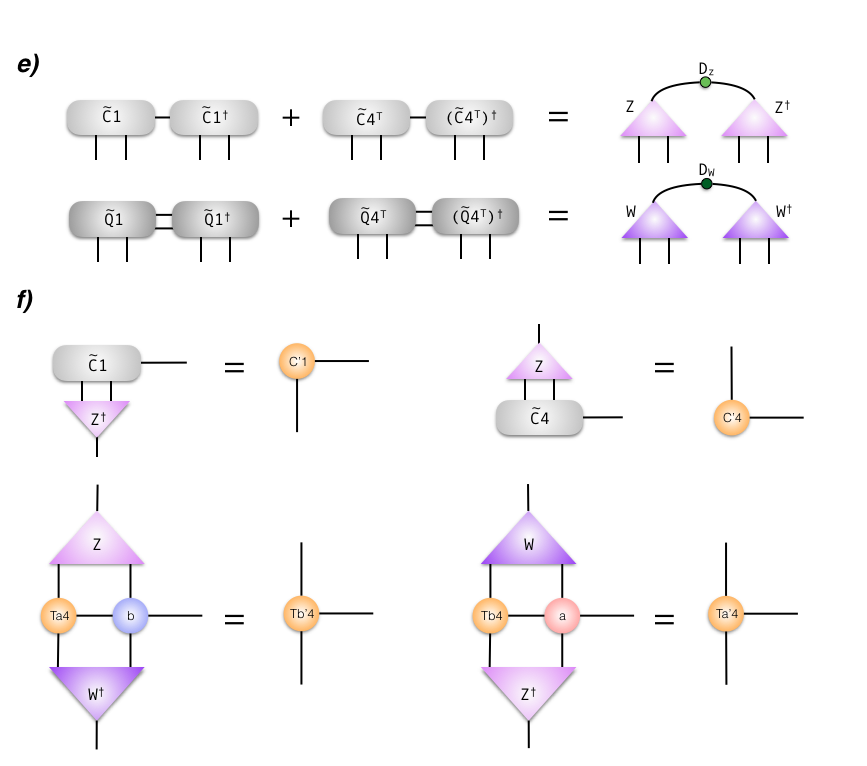
\includegraphics[width=0.75\textwidth]{figures/fig513.png}
	\caption[The picture of the main idea of itebd.]{The red and blue tensor denotes on \textit{odd} and \textit{even} sites. The yellow one are time evolution operators $e^{-\tau H_{k,k+1}}$, $e^{-\tau H_{k+1,k}}$}
	\label{fig512}
\end{figure}

\section{Obtain States from PESS}
\label{pessctm}
CTM with PESS.

